\chapter{OVERVIEW ABOUT BAA TRAINING VIETNAM}

\renewcommand{\headrulewidth}{0.5pt}
\renewcommand{\footrulewidth}{0.5pt}
\thispagestyle{plain}
\pagestyle{fancy}
\fancyhf{}
\fancyhead[L]{\textbf{CHAPTER 2}}
\fancyhead[R]{\textbf{Graduate Report}}
\raggedright
\fancyfoot[L]{From: Nguyen Van Anh Tuan}
\fancyfoot[R]{Page \thepage}

\section{History Of Formation And Development}
    BAA Training Vietnam is a subsidiary of BAA Training - one of the leading aviation training center in Northern Europe. 
    Specializes in providing training and training programs for pilots. \\ 
    \begin{figure}[H]
        \centering
        
\includegraphics[width=0.6\linewidth]{img/company-logo.png}
        \caption{BAA Training Vietnam logo}
    \end{figure}
    In 2018, BAA Training targets the Vietnamese market and establishes a headquarters in Vietnam with the goal of establishing 
    a quality aviation training organization with a training program based on EASA's quality standards - 
    European Aviation Safety Agency, for students from inexperienced flying to training to upgrade the captain. BAA Training 
    certifications are approved by the CAAV.
    \begin{itemize}
        \item \textbf{Address:} 99 Le Van Viet street, Tang Nhon Phu A ward, District 9, Ho Chi Minh city, postal address 71207
        \item \textbf{Hotline:} +84 28 389 739 39
        \item BAA Training Vietnam is CAAV approved ATO providing EASA standard aviation training solutions in Asia-Pacific region.
    \end{itemize}
    \begin{figure}[H]
        \centering
        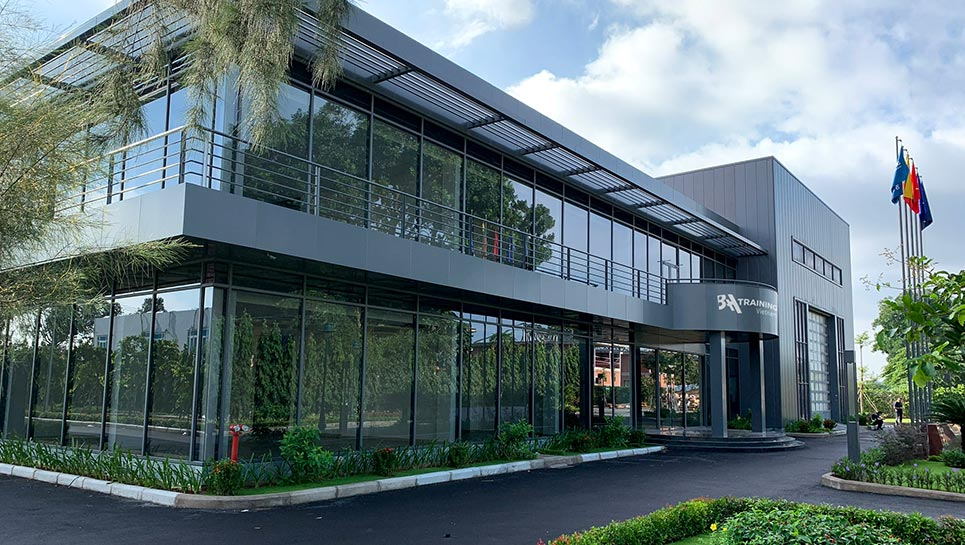
\includegraphics[width=0.6\linewidth]{img/company.jpg}
        \caption{Headquarter of BAA Training Vietnam}
    \end{figure}

\section{Field Of Activity}
    BAA Training Vietnam specializes in providing training services ATPL - Transport pilot license for pilots with CPL certificates. 
    This is a course for pilots who want to work for airlines because according to regulations, a pilot's license is required to fly 
    a transport aircraft to control aircraft for airlines. Moreover, if there is no need to work for the Airline, you can still study 
    according to your wishes. \\ 
    \vspace{3mm}
    In addition, BAA Training Vietnam also provides an integrated training program ATPL(A) for students who do not have flight experience. 
    With this program, upon completion, students will receive an ATPL Frozen license which includes a CPL certificate, instrument flight rating 
    on IR multi-engine aircraft and ATPL theory. In order to prepare students with the necessary knowledge of the job of flying an aircraft, 
    they can control commercial multi-engine aircraft through theoretical, practical and coordinated training with a multi-member MCC crew. \\ 
    \vspace{3mm}
    BAA Training Vietnam also provides Type Rating training services for Airbus A320, Boeing 737 NG, ATR 42/72 aircraft. After completing the 
    course, students will receive a rating for the type of aircraft corresponding to the type of aircraft that the student takes the assessment test. \\ 
    \vspace{3mm}
    In addition, there are training programs specifically designed for airlines at the request of the airline and a number of other training 
    services such as captain promotion, periodic assessment of pilot capacity, experience flight test.

\section{Organizational Structure}
    BAA Training Vietnam has a professional organizational structure with highly qualified and experienced human resources to ensure that the output 
    quality of students fully meets the standards prescribed for this position. pilots' names as well as company performance.
    \begin{figure}[H]
        \centering
        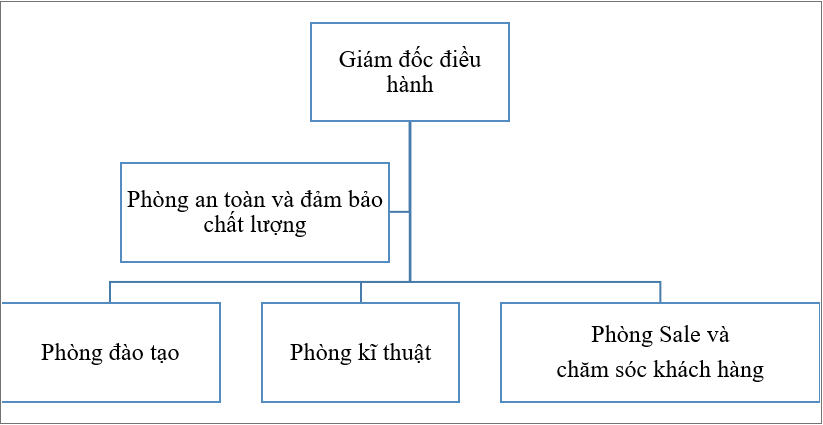
\includegraphics[width=0.6\linewidth]{img/structure.PNG}
        \caption{Organisational structure diagram BAA Training Vietnam}
    \end{figure}
    \subsection{Managing Director}
        To be the legal representative of BAA Training Vietnam on the legal side, to sign the contract and to be the spokesperson for the company. \\ 
        \vspace{3mm}
        Responsible for managing all business activities to ensure that these activities comply with the provisions of Vietnamese law, the guidance 
        of the Ministry of Transport, the Civil Aviation Administration of Vietnam as well as legal documents. \\ 
        \vspace{3mm}
        At the same time, he is responsible for running the company's activities, reviewing and recruiting personnel and appointing the positions of 
        Heads of Training, Technical, Sales and Customer Care departments. \\ 
        \vspace{3mm}
        In addition, the CEO also performs other obligations and powers specified in the company's internal documents.
    \subsection{Quality Assurance Department}
        The main task is to ensure that the company's activities always comply with the quality regulations issued by BAA Training Vietnam internally 
        and required by the Civil Aviation Authority of Vietnam. \\ 
        \vspace{3mm}
        Along with that, it is a tool to support the CEO in formulating policies and standards for aviation training, company operation or human 
        resource quality.
    \subsection{Training Department}
        Develop training standards according to the requirements specified in the aviation safety regulations - Section 7 on Airline Officer Licenses. \\ 
        \vspace{3mm}
        Responsible for training, training students and supervising the company's training program to ensure service quality, detect hazards in the 
        process of operation. \\
        \vspace{3mm}
        BAA Training Department includes: 
        \begin{itemize}
            \item Head of training
            \item Flight instructor
            \item Ground instructor
            \item Training and service development department
        \end{itemize}
    \subsection{Technical Department}
        Ensure that the training equipment at the company meets technical standards and is always in stable condition through regular inspection and 
        evaluation activities. When detecting errors, they must notify the Executive Director for timely resolution. In addition, the technical department 
        is also responsible for preparing equipment for students before the lesson begins.
    \subsection{Sales And Customer Care Department}
        Consulting and supporting students to learn information about the company's services. Answer questions and complaints of students during the learning 
        process. Support students when needed and manage the company's social networking sites to reach and attract new students.

\section{Main Resources}
    \subsection{Infrastructure}
        BAA Training Vietnam's training facility is built on a 3000 $m^2$ site with 2 floors. \\ 
        \vspace{3mm}
        The first floor includes:
        \begin{itemize}
            \item 2 Simulated cockpit devices A320, technical and maintenance department, spare parts warehouse
            \item 1 Storage room
            \item 4 Classrooms
            \item 1 Dining room
            \item 1 Meeting room
        \end{itemize}
        The second floor includes:
        \begin{itemize}
            \item 4 Offices 
            \item 5 Briefing – room
            \item 1 ATP training room, air transport pilot theory 
            \item 5 Classrooms
            \item 1 Living room
        \end{itemize}
    \subsection{Training Equipment}
        Training equipment at BAA Training Vietnam includes:
        \begin{itemize}
            \item Flight simulator Airbus A320neo, Airbus A320ceo
            \item Flight training equipment CAE 400XR
            \item Personal computers and tablets for students and pilots
            \item Projector, headset, recording software for learning
            \item 
            Other equipment: lights, air conditioners, writing boards, fire prevention and fighting systems...
        \end{itemize}
        \begin{figure}[H]
            \centering
            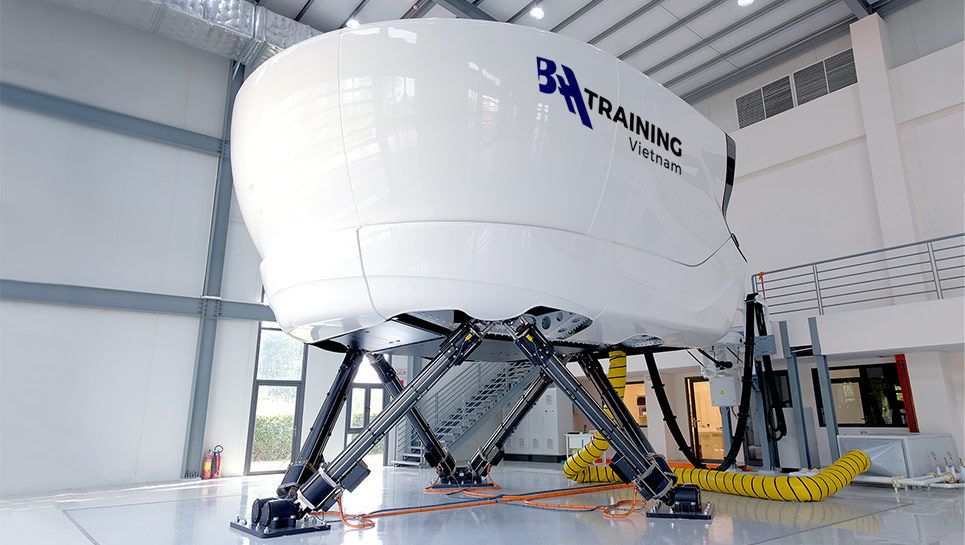
\includegraphics[width=0.6\linewidth]{img/flight-simulator.jpg}
            \caption{Flight simulator device}
        \end{figure}

\section{Performance results 2019 - 2020}
    Participating in the Vietnamese market since 2018 but BAA Training Vietnam officially went into operation in 2019 after completing the construction 
    and assembling of equipment. Therefore, the operation time of the center up to now is less than 2 years. However, the operating results of BAA 
    Training Vietnam still have a good signal. \\ 
    \vspace{3mm}
    In the past year 2020, BAA Training Vietnam was granted the UPRT training certificate - Upset Prevention and Recovery Training for the first A320 
    airplane in Vietnam for the purpose of improving the pilot's ability as well as the level of flight safety during flight performance.